\chapter{Arquitectura}
\label{chap:Arquitectura}

 \textbf{
   \begin{tabular}{|l|}
   \hline
   DRAFT                                                              \\
   \hline
   \end{tabular}
 }

 Este capítulo describe la arquitectura general del sistema, el 
 protocolo de comunicación con el servidor MASSIM, la 
 arquitectura interna de cada agente, incluyendo la entrada y
 salida de datos, las fases de preprocesamiento de las percepciones,
 el esquema de representacion de conocimiento utilizada y el proceso 
 deliberativo realizado por cada agente.
 
%--------------------------------------------------------ARQ SISTEMA-%
\section{Arquitectura del sistema}
\label{sec:arquitectura_sistema}

 El sistema \texttt{\textbf{d3lp0r}} consiste del conjunto de procesos 
 Agentes y el proceso Servidor de Percepciones. 
 Los Agentes tienen como componentes principales al módulo principal, 
 que dirije la lógica de control del agente, los módulos de 
 comunicación con el servidor MASSim y el Servidor de Percepciones, 
 y los módulos de establecimiento de creencias y deliberacion.
 El Servidor de Percepciones esta implementado en un único módulo, y 
 tiene como componentes principales la lógica de control y el protocolo 
 de comunicación. 

 % ORIGIN: report
 El programa principal del agente esta implementado en Python y maneja
 toda comunicación con los servidores, parseo de los mensajes XML, 
 procesamiento de la información contenida en las percepciones para 
 transformarlas a un formato adecuado para su aserción en la base de 
 conocimiento del agente, y la generación del XML que representa las 
 acciones que toma el agente y es enviado al servidor MASSim. 

 % ORIGIN: report
 La inicialización del agente consiste en la apertura de la conexión al 
 servidor MASSIm y la subsiguiente autentificación, la apertura de la 
 conexión al Servidor de Percepciones, y la inicialización del motor 
 Prolog.
 Luego de la fase de inicialización se ingresa al bucle principal, en 
 el cual se reciben y parsean mensajes del servidor MASSim y se responde
 a ellos de manera adecuada.  

 Al recibir un mensaje de tipo \texttt{sim-start}, la información 
 presente en el mensaje tal como el rol del agente y los parametros
 de la simulación se asertar en la base de conocimiento del agente y 
 se inicia el ciclo de percibir-actuar.

 Cada iteracion del bucle de percibir-actuar espera un mensaje de tipo
 \texttt{request-action} desde el servidor MASSim y parsea el XML para
 transformarlo en un diccionarion (arreglo asociativo) de Python. 
 Los elementos de la percepción se separan en una sección ``publica'', 
 la cual es enviada al Servidor de Perceciones, y otra ``privada''.

 A continuación el agente enviará la sección pública de su percepción 
 al Servidor de Percepciones y espererá la ``percepción global'' que 
 contendrá el resto de la información percibida por el equipo. 
 La percepción global se unirá con su propia, y será asertada en su 
 b ase de conocimiento, estableciendo sus creencias. 

 El módulo de decisión implementado en Prolog es consultado para 
 determinar la siguiente acción que ejecutará el agente. 
 Una vez que el flujo de control retorna al programa Python con el 
 resultado de la fase deliberativa, el mensaje XML correspondiente es 
 generado y enviado al servidor MASSim.   

 \begin{figure}[ht]
 \centering
 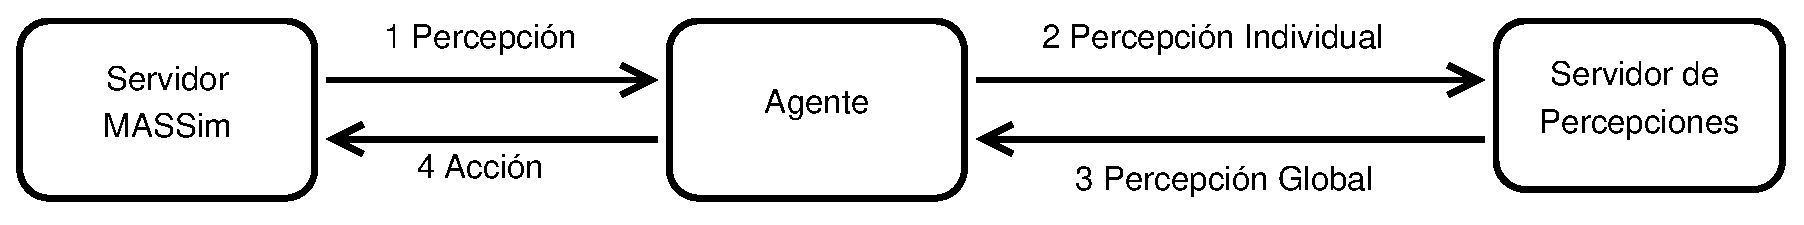
\includegraphics[scale=.5]{graficos/eps/system_architecture.eps}
 \caption{Diagrama de la secuencia de acciones de cada ciclo de la simulación.}
 \label{fig:system_architecture}
 \end{figure}

%---------------------------------------------CONEXION MASSIM-SERVER-%
\section[Conexión con el MASSim Server]
 {Conexión del Agente con el Servidor MASSim}
 \label{sec:conexion_massim}

 El protocolo de comunicación con el servidor MASSim especificado por 
 el enunciado del concurso MAPC define que los agentes y el servidor 
 intercambian mensajes en formato XML codificados por UTF-8, con un 
 byte nulo para indicar el final del mensaje. 

%--------------------------------------------PROTOCOLO MASSIM-SERVER-%
\subsection[Protocolo del MASSim Server]
 {Protocolo de comunicación con el servidor MASSim}
 \label{sub:protocolo_massim}

 Los agentes de cada equipo se ejecuta localmente, mientras que el entorno
 simulado, sobre el cual los agentes de todos los equipos realizan acciones,
 corria en un servidor remoto.

 Los agentes se comunican con el servidor del concurso a traves de un socket 
 TCP/IP estandard con una interface de socket, sobre el cual intercambiaban 
 mensajes XML.
 Los mensajes son documentos bien formados de XML, los mensajes mal formados 
 son ignorados por el servidor de simulación. 

 Cada torneo consiste de un numero de partidos.
 Una partido es una secuencia de simulaciones en las cuales varios equipos de 
 agentes compiten en varios escenarios del entorno.
 Desde el punto de vista del agente, el torneo consiste de una secuencia de 
 simulaciones, en distintos escenarios, contra distintos equipos.

 El torneo se divide en tres fases:

 \begin{enumerate}
 \item La fase inicial,
 \item la fase de simulación,
 \item la fase final.
 \end{enumerate}

 Durante la fase inicial, los agentes se conectan al servidor de simulación y 
 se identifican mediante un nombre y una contraseña (mensaje 
 \texttt{AUTH-REQUEST}) que puede resultar en exito o fracaso.
 Luego de una autentificación exitosa, los agentes deberán esperar a que 
 comienze la primera simulación del torneo.
 La figura \ref{fig:fase_inicial} muestra la fase inicial.

 \textbf{
 \begin{tabular}{|l|}
 \hline
 FIGURA DE FASE INICIAL \\
 \hline
 \end{tabular}
 }

 En cada paso de la simulación el agente recibe una percepción de su entorno 
 (mensaje \texttt{REQUEST-ACTION}) y debe responder con la  acción (mensaje 
 \texttt{ACTION}).
 El agente debe entregar su respuesta antes de un tiempo determinado.
 El mensaje de la acción debe contener el identificador de la acción y sus 
 parámetros. 
 La figura \ref{fig:fase_simulacion} muestra la fase de simulación. 

 \textbf{
 \begin{tabular}{|l|}
 \hline
 FIGURA DE FASE SIMULACION \\
 \hline
 \end{tabular}
 }

 Cuando la simulación concluye, los agentes participantes reciben una 
 notificación de su conclusión (mensaje \texttt{SIM-END}) que incluye el 
 resultado de la simulación. 
 Todo agente que actualmente no participa en una simulación debe esperar hasta 
 que el servidor de simulación les notifique que o bien comienza una simulación 
 o que el torneo concluye. 

 Al final del torneo, todos los agentes reciben una notificación (mensaje 
 \texttt{BYE}) y a continuación el servidor de simulación cerrará las 
 conexiones a los agentes
 La figura \ref{fig:fase_final} muestra la fase final. 

 \textbf{
 \begin{tabular}{|l|}
 \hline
 FIGURA DE FASE FINAL \\
 \hline
 \end{tabular}
 }

 \subsubsection{Reconexión}
 \label{sub:reconexion_massim} 

 Si un agente pierde su conexión con el servidor de simulación, el torneo 
 continúa sin interrupción, y las acciones del agente desconectado se 
 consideran vacias (de tipo \texttt{skip}). 
 Los agentes son responsables de mantener la conexión al servidor de simulación 
 y en el caso de una interrupción, se les permite reconectarse.
 Los agentes se reconectan realizando la misma secuencia de pasos que al 
 principio del torneo.
 Después de establecer la conexión con el servidor de simulación, envia un 
 mensaje \texttt{AUTH-REQUEST} y recibe un \texttt{AUTH-RESPONSE}. 
 Luego de una autentificación exitosa, el servidor envia un mensaje 
 \texttt{SIM-START} al agente. 
 Si el agente participa en una simulación que esta corriendo, el mensaje 
 \texttt{SIM-START} se envia inmediatamente después del mensaje 
 \texttt{AUTH-RESPONSE}.
 De lo contrario el agente esperará hasta que comienze la próxima simulación en 
 la cual participa.
 En el siguiente paso cuando el agente debe seleccionar una acción, recibe un 
 mensaje \texttt{REQUEST-ACTION} estandard conteniendo la percepción del agente 
 ese turno y la simulación procede de manera normal.
 La figura \ref{fig:reconexion_massim} muestra el protocolo de reconexión. 

%---------------------------------------------------FORMATO MENSAJES-%
\subsection{Formato de mensajes}
 \label{sub:formato_mensajes}

 \textbf{
 \begin{tabular}{|l|}
 \hline
 TODO : entro en detalle con la descripcion de los mensajes? \\
 \hline
 \end{tabular}
 }

\subsubsection{\texttt{AUTH-REQUEST}}

\subsubsection{\texttt{AUTH-RESPONSE}}

\subsubsection{\texttt{SIM-START}}

\subsubsection{\texttt{SIM-END}}

\subsubsection{\texttt{BYE}}

\subsubsection{\texttt{REQUEST-ACTION}}

\subsubsection{\texttt{ACTION}}

  \begin{verbatim}
  <?xml version="1.0" encoding="UTF-8" standalone="no"?>
    <message type="action">
      <action id=\"ID\" type=\"TYPE\"/>
    </message>\0
  \end{verbatim}
  
  En el caso de las acciones que requieren un parámetro adicional, la
  representación es:
  
  \begin{verbatim}
  <?xml version="1.0" encoding="UTF-8" standalone="no"?>
    <message type="action">
      <action id="ID" param="PARAM" type="TYPE"/>
    </message>\0
  \end{verbatim}
  
  donde {\tt ID} es el identificador de mensaje enviado por el servidor
  MASSim en la percepcion, {\tt TYPE} es el tipo de acción y {\tt PARAM}
  es el parametro. 
  
  {\tt TYPE} puede ser uno de:
  
  \begin{itemize}
  \item \tt{skip}
  \item \tt{goto}
  \item \tt{attack}
  \item \tt{parry}
  \item \tt{probe}
  \item \tt{survey}
  \item \tt{inspect}
  \item \tt{repair}
  \item \tt{recharge}
  \item \tt{buy}
  \end{itemize}

%---------------------------------------------------------ARQ AGENTE-%
\section{Arquitectura del agente}
 \label{sec:arquitectura_agente}

 Esta sección tiene el objetivo de analizar el diseño y estructura de 
 un agente individual.

%-------------------------------------------------------------DISEÑO-%
\subsection{Diseño general}
 \label{sub:diseno_general}
 
 % ORIGEN: marcov 
 El programa agente presenta una estructura simple en cuanto a su
 división.
 La interacción con el entorno y el procesamiento inicial de la
 información recibida finalizan con la generación de una serie de
 creencias que son incorporadas a la base de conocimiento mantenida por
 el agente.
 Este conjunto de creencias es empleado posteriormente por el módulo
 encargado de tomar decisiones.
 La forma en que se estructuran los componentes principales es
 detallada a continuación.

 % ORIGEN: report
 El agente parsea las opciones pasadas por linea de comando al iniciar 
 que determinaran sus paremetros de comportamiento.
 Entre ellos estan los detalles de autentificación que utilizará con 
 el MASSim server (nombre de usuario y contraseña), si esta habilitado 
 el registro de eventos y su nivel de verbosidad, la ubicación en la 
 red del Servidor de Percepciones, y si el agente operará en modo 
 ``dummy'' (en el cual no utiliza argumentación en el proceso 
 deliberativo) o no. 

 % ORIGEN: report
 El mensaje de inicio de simulación es enviado por el MASSim server 
 cada vez que un agente se conecta.  
 
 Los posibles tipos de mensajes son \texttt{sim-start}, \texttt{sim-end}, 
 \texttt{request-action} y \texttt{bye}. 

 Para cada solicitud de acción, la cual incluye la percepción del 
 agente para ese turno, el agente procesará el mensaje, enviando la 
 información que desea compartir con los demás agentes del equipo al 
 servidor de Percepciones, reincorporá la respuesta del 
 Servidor de Percepciones a su base de conocimiento, iniciará el 
 proceso deliberativo para llegar a una decisión sobre cual acción 
 tomar, y finalmente enviará un mensaje representando su decisión al 
 servidor MASSim.   

\subsubsection{Estructura básica del agente}
 \label{subsub:estructura_basica_de_agente}
  
 El programa principal del agente es el encargado de manejar la
 comunicación con los servidores, tanto el del juego como el de
 percepciones (presentado a continuación).
 También es responsable de parsear y procesar la información contenida
 en la percepción para darle el formato interpretado por la base de
 conocimientos, y enviar la acción que ha sido elegida por el módulo
 de toma de decisiones.
 
 \begin{figure}
 \centering
 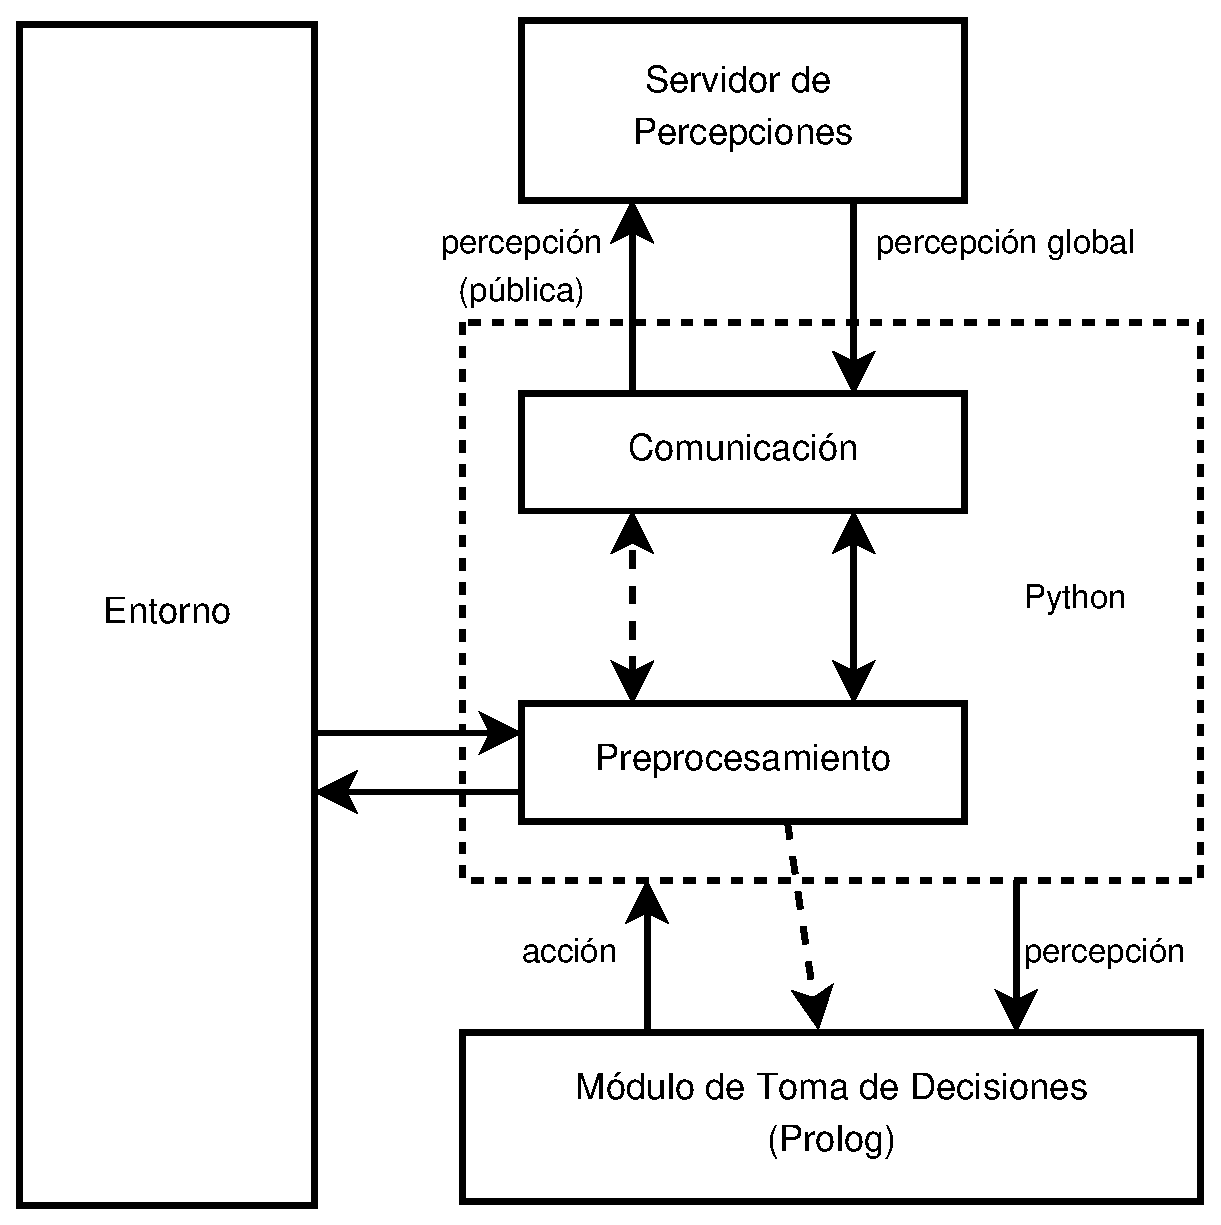
\includegraphics[scale=.4]{graficos/eps/agent_architecture.eps}
 \caption{Diagrama de la arquitectura del agente. Las líneas punteadas
 representan el flujo de control, y las líneas contínuas representan el
 flujo de datos.}
 \label{fig:architecture}
 \end{figure}
 
 El servidor de percepciones (SP) es un programa independiente,
  encargado de unificar las percepciones de todos los agentes que se
 encuentran en ejecución.
 Recibe sus percepciones individuales y retorna a cada uno de ellos el
 conjunto de datos que aún no poseen, de manera que todos los agentes
 del equipo cuenten con la misma información en cuanto al estado del
 escenario.
  
 En cada iteración de la simulación, el agente recibe un mensaje por
 parte del servidor del juego, el cual contiene la información
 asociada a la percepción del turno en disputa.
 Este mensaje es parseado y traducido en una estructura que permite
 manipular los datos con mayor facilidad.
 Los datos son divididos en dos conjuntos, uno ``público'', el cual es
 compartido con los demás agentes del equipo, y uno ``privado''.
 La sección pública de datos es compartida a través del mencionado
 servidor de percepciones.
 
 El agente une entonces su propia percepción con la percepción global
 recibida del servidor de percepciones, y genera un único conjunto de
 datos.
 Esta información es incorporada a la base de conocimientos,
 estableciendo nuevas creencias para el agente.
 
 El módulo de toma de decisiones, analizado en la sección
 \ref{sec:arquitectura_bdi}, es el que implementa el modelo BDI
 respetado por el agente.
 Este módulo es consultado en cada iteración para obtener la próxima
 acción a ser ejecutada.
 Una vez que el flujo de control retorna al programa principal, la
 acción seleccionada es enviada al servidor del juego.
  
\subsubsection{BASE DE CONOCIMIENTO}

%----------------------------------------------------------------BDI-%
\subsection{Arquitectura BDI} 
 \label{sub:arquitectura_bdi}

 El módulo de toma de decisiones es consultado por el programa
 principal, obtiene la próxima acción a ser ejecutada, y la retorna
 para que pueda ser enviada.
 Esta es una secuencia que se reitera en cada uno de los turnos de la
 simulación, con una característica: cuando es necesario plantear y
 planificar una nueva meta, intervienen una serie de componentes
 especiales, que difieren de aquellos involucrados cuando se cuenta con
 una meta ya planificada.
 Cada uno de estos componentes es descrito en esta sección.
 
 \begin{figure}[ht]
 \centering
 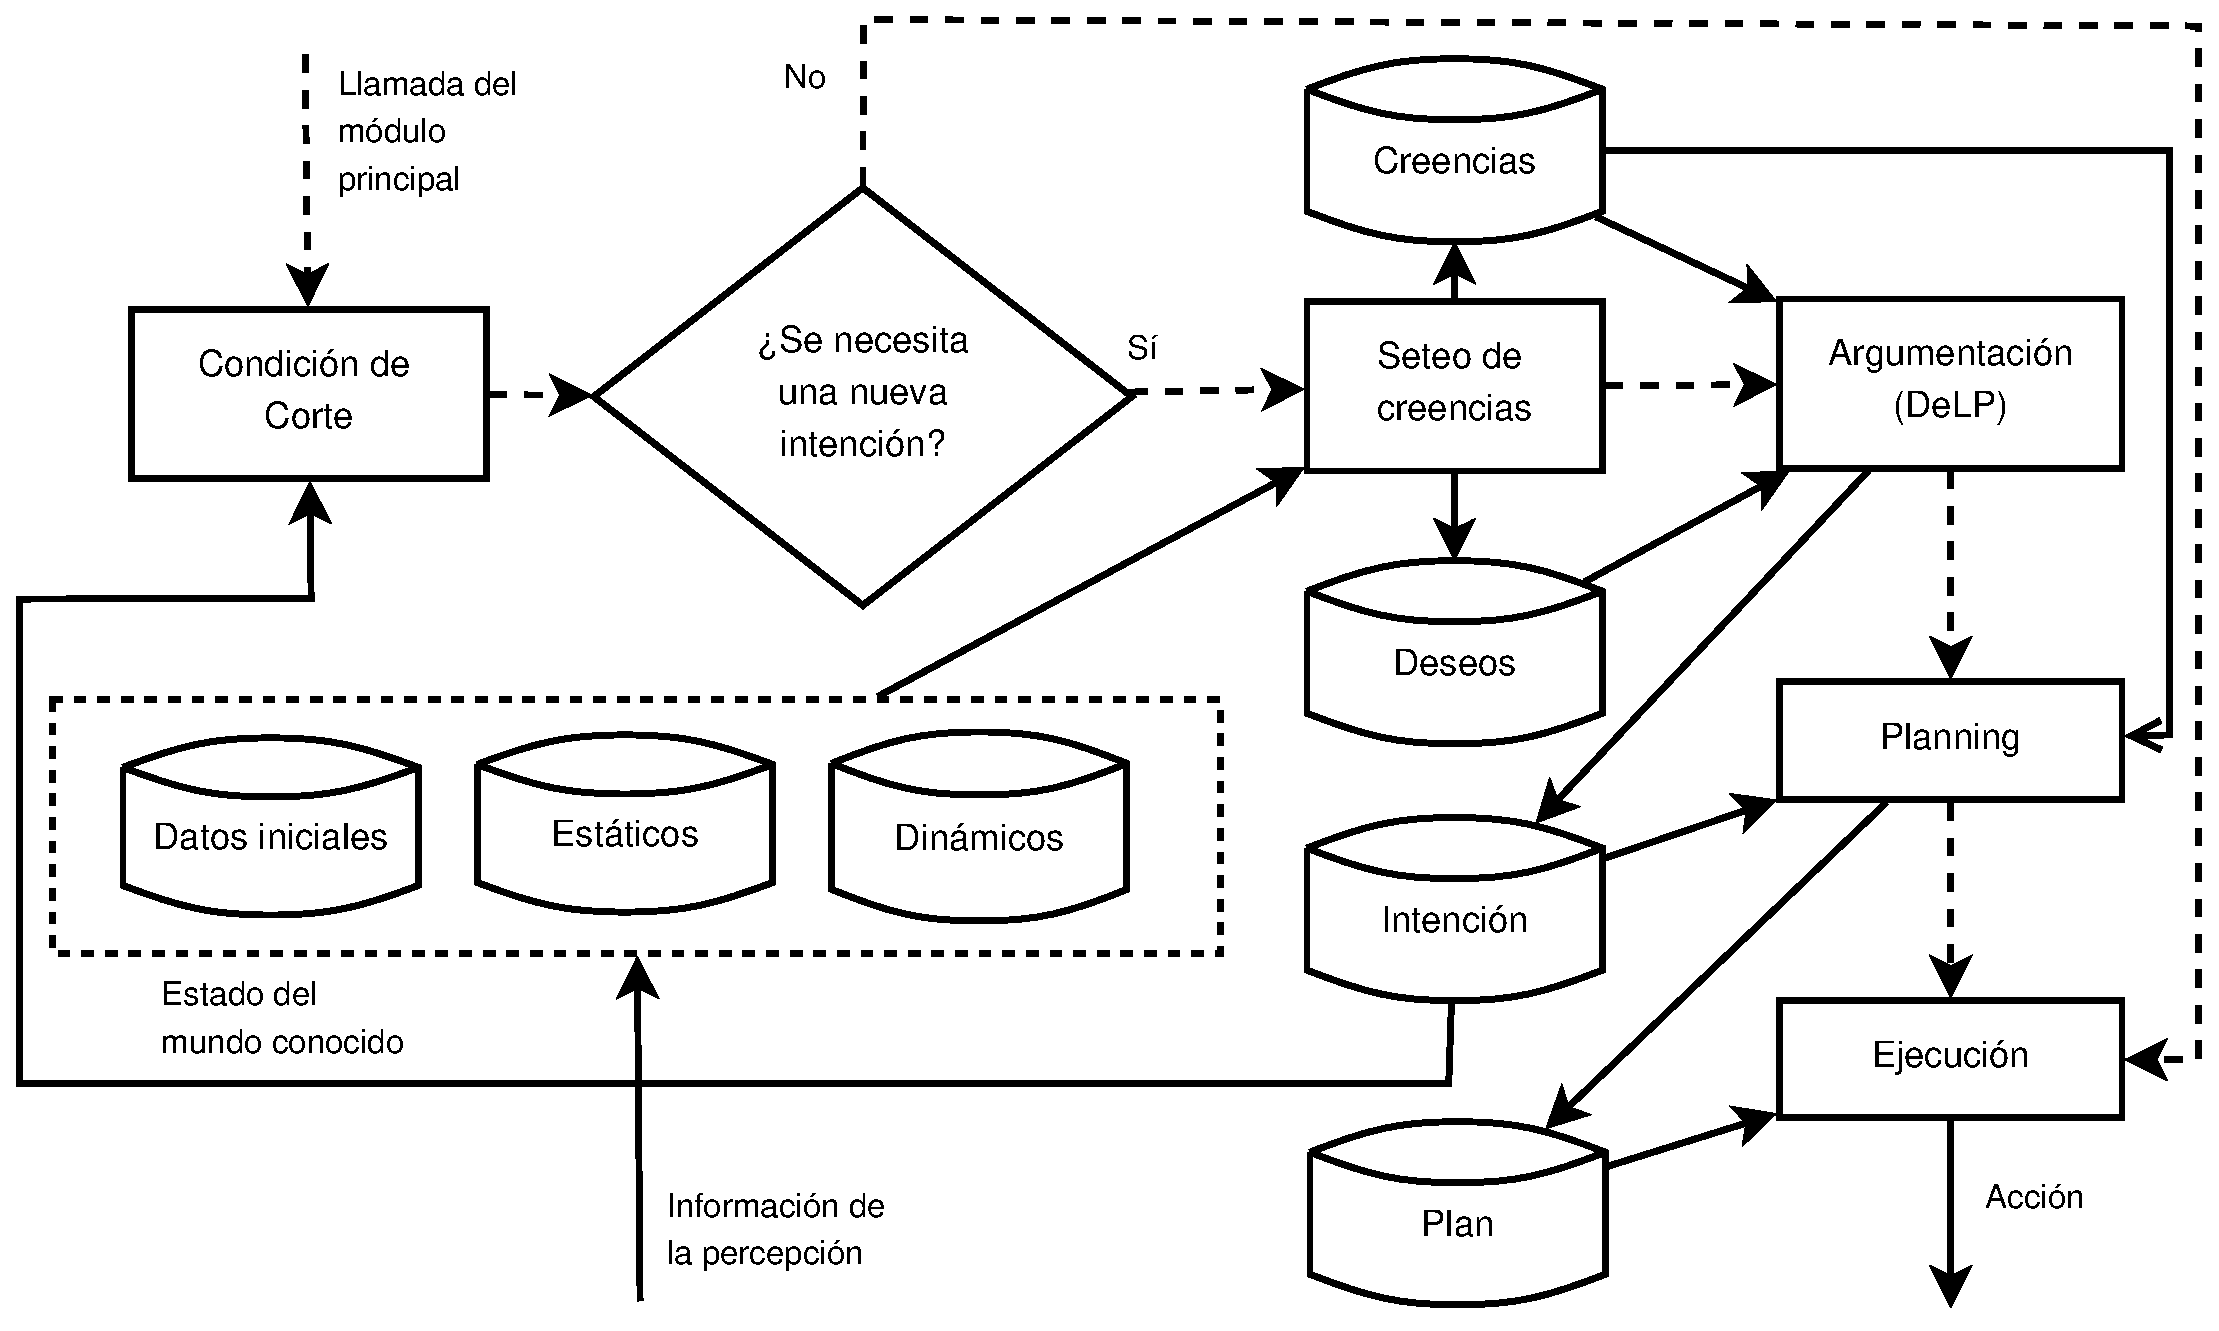
\includegraphics[scale=.3]{graficos/eps/agent_prolog.eps}
 \caption{Diagrama de la arquitectura interna del agente,
 particularmente todo lo relacionado con la toma de decisiones, hecha
 en Prolog.
 Las líneas punteadas representan el flujo de control, y
 las líneas contínuas representan el flujo de datos.}
 \label{fig:agent_prolog}
 \end{figure}
  
\subsubsection{Seteo de creencias}
 \label{subsub:seteo_de_creencias}
  
 El seteo de creencias es llevado a cabo cada vez que el agente se
 dispone a seleccionar una nueva intención.
 Incluye la generación de aquellos datos que pueden permitir al agente
 realizar una elección lo más acertada posible.
 Se trata de inferencias realizadas en base al estado del escenario, es
 decir, aquella información que, como fue mencionado, es almacenada en
 \texttt{b/1}.
 No forma parte de este proceso la información proveniente de la
 percepción, ya que el estado del entorno es actualizado en cada turno
 de manera previa.
 Como se detalla a continuación, distintos tipos de creencias pueden
 pueden estar relacionadas a distintos factores, como el rol del
 agente, su estado, o los deseos en análisis.
  
 \paragraph{Creencias generales}
  
 Existe un conjunto de creencias que resultan de utilidad general para
 todo el proceso de decisión.
 Por esta razón, son las primeras en ser calculadas y almacenadas
 durante el seteo de creencias.
 Entre los datos incluidos, se encuentra el puntaje que están aportando
 las zonas armadas, la diferencia de puntos que puede producirse si el
 agente abandona su posición (ambos puntajes calculados utilizando una
 versión propia y optimizada del \textit{algoritmo de coloreo} de la
 competencia, que a su vez será reutilizado en la etapa de resolución
 de conflictos), y la seguridad que brindan las distintas ubicaciones
 posibles en cuanto a la presencia de agentes saboteadores enemigos.
  
 \paragraph{Deseos}
  
 Como se detallará en la sección siguiente, el proceso de toma de
 decisión conlleva el pesaje de todos los posibles deseos del agente, y
 la posterior selección del más beneficioso.
 Dichos deseos surgen de un conjunto predefinido, y pueden, según sea
 el caso, estar instanciados con diferentes entidades del juego, como
 agentes o nodos. Para que esta selección sea posible, es necesario
 determinar, de manera previa, qué deseos e instanciaciones son
 realmente factibles, y por lo tanto deben ser tenidos en cuenta, y
 cuales pueden ser descartados anticipadamente.
 Para esto se analizan distintas condiciones como, por ejemplo, la
 distancia a un nodo que no ha sido explorado.
 Si el nodo se encuentra a una distancia que supera una cota pre-
 establecida, entonces el deseo de explorar ese nodo no es contemplado.
 Los deseos e instanciaciones considerados factibles son seteados en la
 base de conocimiento.
 
 \begin{verbatim}
   b(posibleExplorar(vertex4)).
 \end{verbatim}
  
 \paragraph{Creencias específicas} 

 % Seteo de beliefs para cada deseo.
  
 Junto con los deseos a ser evaluados, es necesario incluir en la base
 de conocimiento un conjunto de creencias relacionadas a estos deseos.
 Entre las más importantes, se encuentran las distancias que existen
 desde la posición actual del agente a los distintos nodos de interés,
 y la diferencia de puntaje que se produce en caso que el agente se
 desplace a dichas ubicaciones.
 Estos datos resultan fundamentales, ya que afectan directamente la
 valuación que se realiza de cada deseo, y por lo tanto la posterior
 selección.
  
 En esta etapa, también se produce el seteo de datos requeridos
 posteriormente, como son los caminos a los diferentes nodos
 analizados.
 Los algoritmos empleados para la búsqueda de caminos almacenan todos
 los caminos hallados, en forma de secuencia de acciones, de manera que
 la etapa de planificación, ejecutada cuando se ha decidido una
 intención, pueda ser realizada en forma simple e directa.
  
 \paragraph{Creencias especiales} 

 % Seteo de beliefs en caso de agente deshabilitado.
  
 Cuando el agente se encuentra en una situación de peligro, esto es, no
 posee el rol de saboteador y hay un saboteador enemigo en su posición,
 o fue atacado en el turno anterior, el conjunto de creencias seteadas
 se reduce.
 En estos casos, sólo son tenidos en cuenta los nodos vecinos, dado que
 representan las vías de escape más rápidas; son calculadas las
 distancias a estos (en cantidad de turnos), y las diferencias de
 puntaje que produciría el desplazamiento del agente.
 Esto tiene el objetivo de minimizar la cantidad de deseos
 considerados: sólo son evaluadas la posibilidad de permanecer en la
 misma ubicación (si el beneficio en puntaje es considerable), y las
 distintas alternativas de defensa propia que pueden llevar al agente a
 superar el peligro.

%------------------------------------------------------ARGUMENTACION-%
\subsection{Argumentación}
 \label{sub:argumentacion}
  
 Una vez finalizado el seteo de creencias, el agente procede a la
 selección de la próxima intención.
 Para esto, se toma cada uno de los deseos marcados como factibles en
 la base de conocimiento, y se los evalua junto a una serie de
 ``condiciones'' particulares.
 Se considera que existen razones para creer realizables sólo aquellos
 deseos que satisfacen sus condiciones.
 Para estos, se obtiene un valor que representa su peso, en términos
 del beneficio que conllevan para el equipo.
 El deseo que presenta el mayor peso entre los analizados, se convierte
 en la nueva meta del agente, la cual es almacenada hasta ser alcanzada
 o reemplazada.
 
 Tanto la evaluación como el pesaje de los deseos, son llevados a cabo
 empleando \textit{argumentación} en un módulo especial, implementado
 con la ayuda de \textit{DeLP}.
  
\subsection{PLANIFICACION}

\subsection{EJECUCION}
